En el presente capítulo se expone los métodos utilizados para 
conseguir los objetivos específicos detallados en el Capítulo 
\ref{objetivos}. Cada subsección corresponde con cada uno de 
los objetivos en los que se explicará en qué consiste cada 
objetivo de forma más extendida, la herramienta escogida 
para su realización y la justificación de su elección.

\section{Descripción del \textit{Dataset}}

Para la realización de este trabajo se decidió elegir el 
``\textit{Hockey Fight Detection Dataset}'' el cual es un 
conjunto de datos ampliamente utilizado en la investigación 
sobre detección automática de violencia en videos. Fue 
desarrollado por Enrique Bermejo Nievas, Óscar Deniz Suárez, 
Gloria Bueno García y Rahul Sukthankar, y publicado en 2011 
\cite{nievas2011violence}. 
Este dataset fue concebido para abordar la necesidad de 
sistemas capaces de identificar comportamientos agresivos en 
entornos de vigilancia, como prisiones, centros psiquiátricos 
o residencias de ancianos, donde la detección temprana de 
violencia es crucial.

El conjunto de datos consta de 1,000 secuencias de video, 
divididas equitativamente en dos categorías: 500 videos 
que muestran peleas durante partidos de hockey sobre hielo 
y 500 videos sin violencia. Cada video tiene una duración 
aproximada de 1 a 2 segundos y está etiquetado manualmente 
para facilitar su uso en tareas de clasificación supervisada. 
Los videos fueron recopilados de diversas fuentes, incluidos 
sitios web de noticias y plataformas de video en línea, 
asegurando una variedad de escenarios y condiciones de 
iluminación. En la figura \ref{fig:combinedHockey} se muestra 
una comparación de un frame de cada uno de las etiquetas: 

\begin{figure}[h!]%
    \centering
    \subfloat[\centering Frame conteniendo violencia]{{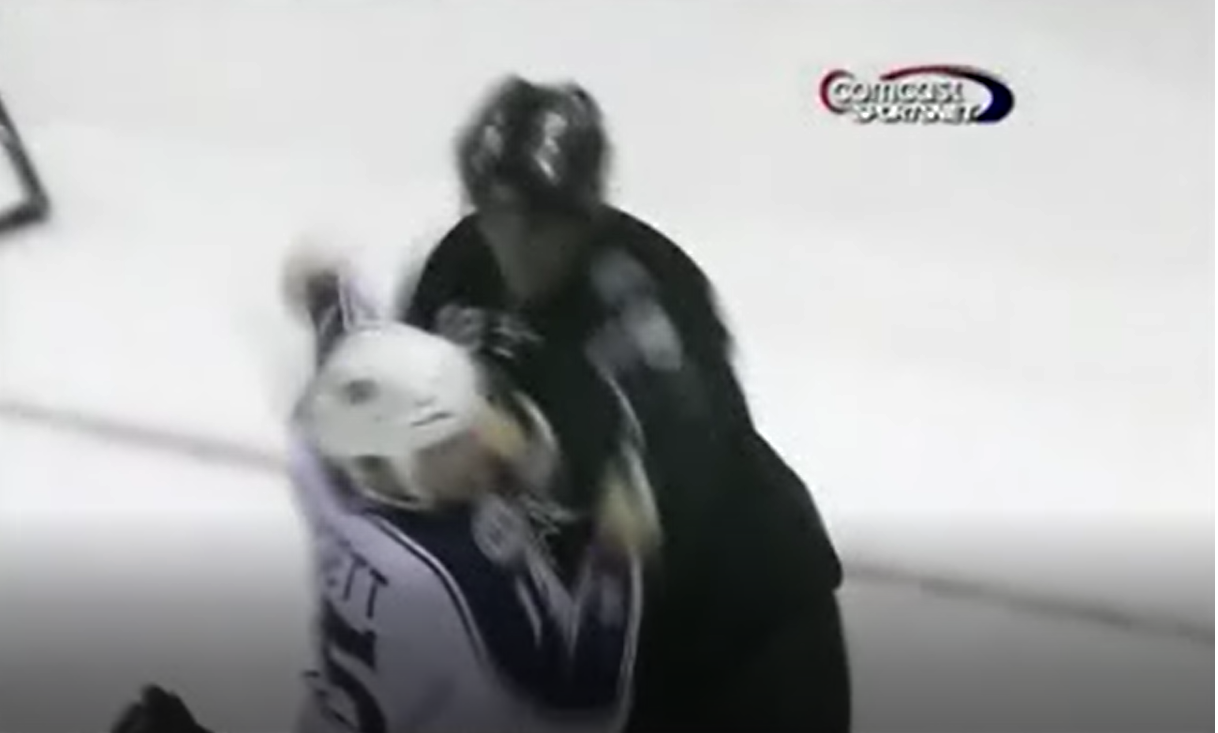
\includegraphics[width=6cm]{images/hockeyFight.png} }}%
    \qquad
    \subfloat[\centering Frame no conteniendo violencia]{{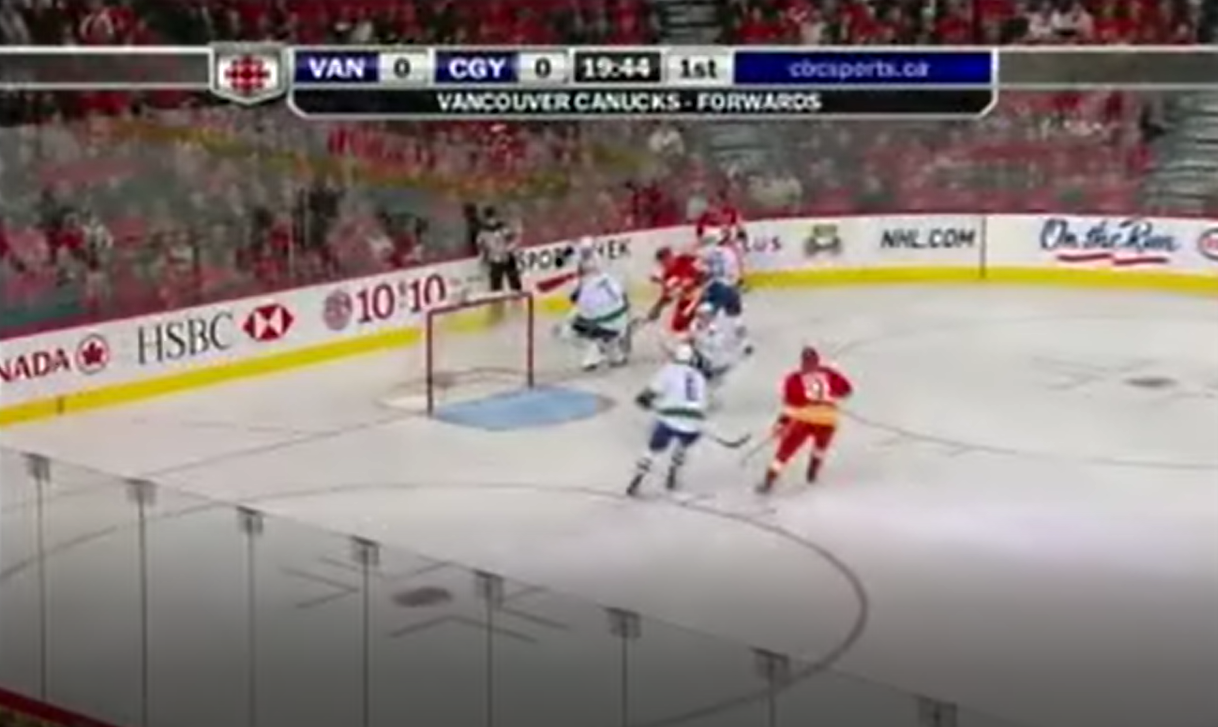
\includegraphics[width=6cm]{images/hockeyNotFight.png} }}%
    \caption{Comparación entre frames con y sin violencia en el ``Hockey Fight Detection Dataset'' }%
    \label{fig:combinedHockey}%
\end{figure}

\section{Pre-procesamiento de la base de datos}

Para preparar los datos del conjunto \textit{Jockey Fights} y 
garantizar su compatibilidad con los modelos de aprendizaje 
profundo utilizados, es necesario el siguiente proceso de 
pre-procesamiento estructurado en varias etapas:

\begin{itemize}
    \item \textbf{Obtención de frames}: Cada video del dataset 
    se descompone en sus respectivos fotogramas (frames) 
    utilizando una frecuencia de muestreo fija. Estos frames 
    fueron almacenados como matrices RGB, representando la 
    información visual en tres canales (rojo, verde y azul), 
    lo cual permitió capturar el contenido visual de cada 
    instante del video.

    \item \textbf{Recorte y redimensionamiento}: Los frames 
    extraídos se redimensionaron a una resolución fija 
    (como 224x224 píxeles), adaptándose así a los 
    requerimientos de entrada de los modelos de red neuronal 
    convolucional (CNN) utilizados en la etapa de extracción 
    de características.

    \item \textbf{Normalización}: Con el objetivo de mejorar 
    la eficiencia del entrenamiento de los modelos, se 
    normalizaron los valores de los píxeles de las imágenes. 
    Esto se realizó escalando los valores del rango [0, 255] 
    al rango [0, 1] o aplicando una normalización estadística 
    basada en la media y desviación estándar de los canales 
    RGB, especialmente útil cuando se emplean modelos 
    preentrenados.

    \item \textbf{Etiquetado de los datos}: A partir de los 
    nombres de los videos y su contexto, se asignaron etiquetas 
    binarias a cada secuencia de imágenes. Los videos fueron 
    clasificados como \textit{violentos} o 
    \textit{no violentos}, y dicha etiqueta fue propagada a 
    todos los frames correspondientes al video, asumiendo 
    homogeneidad del contenido en cada segmento.

    \item \textbf{Filtrado y muestreo}: Para reducir la 
    redundancia y el volumen de datos, se aplicó una 
    estrategia de muestreo temporal, extrayendo únicamente un 
    subconjunto de los frames. Para ello, se propuso un muestreo 
    con reemplazo en donde se seteó un número final de frames 
    y se 
    procedió a obtener un frame cada x de los videos. Se 
    utilizó este algoritmo para manejar el caso en el que el 
    número de frames no sea el mismo no solo para el 
    \textit{dataset} actual, sino para que sea utilizado en 
    otros ejemplares.

\end{itemize}

Este pre-procesamiento es esencial para estandarizar 
los datos, minimizar el ruido y facilitar el posterior 
entrenamiento de los modelos de detección de violencia basados 
en aprendizaje profundo.

\section{Métricas de Evaluación}

Para la evaluación del conjunto de datos 
\textit{Jockey Fights}, se utilizan las siguientes 
métricas de rendimiento:

\begin{itemize}

    \item \textbf{F1-score}: penaliza fuertemente los errores 
    y obliga a capturar los positivos y no tener demasiados 
    falsos positivos.
    \begin{equation}
        \text{F1 Score} = 2 \cdot \frac{\text{Precision} \cdot \text{Recall}}{\text{Precision} + \text{Recall}}
    \end{equation}

    \item \textbf{Tiempo de Inferencia}: Mide el tiempo que 
    el modelo tarda en procesar una secuencia completa o un 
    solo frame. Es crucial para aplicaciones en tiempo real 
    o streaming.

\end{itemize}

\section{Software y hardware utilizados}
A lo largo de toda la experimentación, se utilizará un computador de escritorio con las siguientes características:

\begin{table}[h!]
\centering
\footnotesize
\begin{tabular}{|l|l|}
\hline
\textbf{Componente} & \textbf{Descripción} \\ \hline
Procesador & Procesador	Core i5-10300H 2.50GHz\\ \hline
Memoria RAM & 16GB DDR4 - 3600MHZ \\ \hline
Tarjeta Gráfica & Nvidia RTX 3050 4GB \\ \hline
\end{tabular}
\end{table}

Por otra parte, se utilizó Python, junto con Keras, Sklearn y Tensorflow 
para el desarrollo del \textit{pipeline} en general y el pre y post 
procesamiento de los datos. Para el procesamiento de las imágenes 
se utilizó OpenCV compilado con cudnn para la habilitación 
del uso de tarjeta gráfica. 

\subsection{Evaluación de CNN's para la experimentación}
En 2020, Orhan Yalsin \cite{DataModelos} realizó una resumen 
con algunas métricas para la evaluación de diferentes 
modelos de vanguardia, los cuales son mostrados 
en la Tabla \ref{evaluación}. Nos basamos en sus resultados 
para seleccionar aquellos modelos que son mas eficientes 
tanto en tiempo, espacio y precisión.

\begin{table}[h!]
    \begin{tabular}{|l|r|r|r|r|r|}
    \hline
    \textbf{Model}                                               & \multicolumn{1}{l|}{\textbf{Size}} & \multicolumn{1}{l|}{\textbf{\begin{tabular}[c]{@{}l@{}}Top-1 \\ Accuracy\end{tabular}}} & \multicolumn{1}{l|}{\textbf{\begin{tabular}[c]{@{}l@{}}Top-5 \\ Accuracy\end{tabular}}} & \multicolumn{1}{l|}{\textbf{Parameters}} & \multicolumn{1}{l|}{\textbf{Depth}} \\ \hline
    Xception                                                     & 88 MB                              & 0.790                                                                                   & 0.945                                                                                   & 22,910,480                               & 126                                 \\ \hline
    VGG16                                                        & 528 MB                             & 0.713                                                                                   & 0.901                                                                                   & 138,357,544                              & 23                                  \\ \hline
    VGG19                                                        & 549 MB                             & 0.713                                                                                   & 0.900                                                                                   & 143,667,240                              & 26                                  \\ \hline
    ResNet50                                                     & 98 MB                              & 0.749                                                                                   & 0.921                                                                                   & 25,636,712                               & -                                   \\ \hline
    ResNet101                                                    & 171 MB                             & 0.764                                                                                   & 0.928                                                                                   & 44,707,176                               & -                                   \\ \hline
    ResNet152                                                    & 232 MB                             & 0.766                                                                                   & 0.931                                                                                   & 60,419,944                               & -                                   \\ \hline
    ResNet50V2                                                   & 98 MB                              & 0.760                                                                                   & 0.930                                                                                   & 25,613,800                               & -                                   \\ \hline
    ResNet101V2                                                  & 171 MB                             & 0.772                                                                                   & 0.938                                                                                   & 44,675,560                               & -                                   \\ \hline
    ResNet152V2                                                  & 232 MB                             & 0.780                                                                                   & 0.942                                                                                   & 60,380,648                               & -                                   \\ \hline
    InceptionV3                                                  & 92 MB                              & 0.779                                                                                   & 0.937                                                                                   & 23,851,784                               & 159                                 \\ \hline
    \begin{tabular}[c]{@{}l@{}}Inception\\ ResNetV2\end{tabular} & 215 MB                             & 0.803                                                                                   & 0.953                                                                                   & 55,873,736                               & 572                                 \\ \hline
    MobileNet                                                    & 16 MB                              & 0.704                                                                                   & 0.895                                                                                   & 4,253,864                                & 88                                  \\ \hline
    MobileNetV2                                                  & 14 MB                              & 0.713                                                                                   & 0.901                                                                                   & 3,538,984                                & 88                                  \\ \hline
    DenseNet121                                                  & 33 MB                              & 0.750                                                                                   & 0.923                                                                                   & 8,062,504                                & 121                                 \\ \hline
    DenseNet169                                                  & 57 MB                              & 0.762                                                                                   & 0.932                                                                                   & 14,307,880                               & 169                                 \\ \hline
    DenseNet201                                                  & 80 MB                              & 0.773                                                                                   & 0.936                                                                                   & 20,242,984                               & 201                                 \\ \hline
    NASNetMobile                                                 & 23 MB                              & 0.744                                                                                   & 0.919                                                                                   & 5,326,716                                & -                                   \\ \hline
    NASNetLarge                                                  & 343 MB                             & 0.825                                                                                   & 0.960                                                                                   & 88,949,818                               & -                                   \\ \hline
    EfficientNetB0                                               & 29 MB                              & 0.771                                                                                   & 0.933                                                                                   & 5,330,571                                & -                                   \\ \hline
    EfficientNetB1                                               & 31 MB                              & 0.791                                                                                   & 0.944                                                                                   & 7,856,239                                & -                                   \\ \hline
    EfficientNetB2                                               & 36 MB                              & 0.801                                                                                   & 0.949                                                                                   & 9,177,569                                & -                                   \\ \hline
    EfficientNetB3                                               & 48 MB                              & 0.816                                                                                   & 0.957                                                                                   & 12,320,535                               & -                                   \\ \hline
    EfficientNetB4                                               & 75 MB                              & 0.829                                                                                   & 0.964                                                                                   & 19,466,823                               & -                                   \\ \hline
    EfficientNetB5                                               & 118 MB                             & 0.836                                                                                   & 0.967                                                                                   & 30,562,527                               & -                                   \\ \hline
    EfficientNetB6                                               & 166 MB                             & 0.840                                                                                   & 0.968                                                                                   & 43,265,143                               & -                                   \\ \hline
    EfficientNetB7                                               & 256 MB                             & 0.843                                                                                   & 0.970                                                                                   & 66,658,687                               & -                                   \\ \hline
    \end{tabular}
    \caption{Evaluación de diferentes modelos. Tabla brindada por Orhan Yalcin \protect\cite{DataModelos}. }
    \label{evaluación}
\end{table}

Esta tabla destaca varios modelos notables por su equilibrio entre 
tamaño, cantidad de parámetros y precisión. Entre ellos VGG19 
(si consideramos solo las capas convolucionales), ResNet50, InceptionV3, 
y los EfficientNetBX resultan tener una buena relación entre el peso, el 
número de parámetros y la precisión que estas obtienen, esta última 
siendo de las más altas dentro de todos estos modelos. Se tuvo en 
consideración la ejecución en videos en tiempo real y por ello se necesitó 
que el modelo sea el más pequeño posible evitando perder la precisión. Por 
otra parte, están las MobileNet, las cuales ya han sido utilizadas para el 
procesamiento de imágenes en tiempo real por ser más ligeras, enfocadas a 
ser utilizadas en celulares. Creemos que todas estas redes eran aptas para 
este problema y pasarán a ser evaluadas en el siguiente capítulo, en base 
al primer \textit{dataset} mencionado anteriormente. \\

Por otra parte, en un trabajo previo de mi autoría, titulado ``Machine 
Learning Pipeline Para el Etiquetado Automático en Imágenes de Especies de 
Peces Peruanos''\cite{Madera2024}, se experimentó con todas las 
redes anteriormente mencionadas para la tarea de clasificación de imágenes 
de peces peruanos. La tabla \ref{table:data1} referencia los resultados 
obtenidos en aquella experimentación:

\begin{table}[h!]
    \footnotesize
    \centering
    \begin{tabular}{|c|c|c|c|c|c|c|}
    \hline
    \textbf{} & \textbf{\begin{tabular}[c]{@{}c@{}}Precisión\\en\\training\end{tabular}} & \textbf{\begin{tabular}[c]{@{}c@{}}Precisión \\ en \\ validation\end{tabular}} & \textbf{\begin{tabular}[c]{@{}c@{}}Precisión \\ en \\testing\end{tabular}} & \textbf{\begin{tabular}[c]{@{}c@{}}Perdida \\ final en \\ training\end{tabular}} & \textbf{\begin{tabular}[c]{@{}c@{}}Velocidad \\ por batch\\ (8 \\imágenes) \\ en ms\end{tabular}} & \textbf{\begin{tabular}[c]{@{}c@{}}Número \\ de\\ épocas\end{tabular}} \\ \hline
    \textbf{Vgg19} & 0.9193 & 0.9928 & 0.9926 & 0.2299 & 71 & 21 \\ \hline
    \textbf{Resnet50} & \textbf{0.9596} & \textbf{0.9993} & 0.9950 & 0.1282 & 52 & 14 \\ \hline
    \textbf{\begin{tabular}[c]{@{}c@{}}Inception\\V3\end{tabular}} & 0.7362 & 0.6620 & 0.6681 & 0.6901 & 42 & 40 \\ \hline
    \textbf{\begin{tabular}[c]{@{}c@{}}MobileNet\\V2\end{tabular}} & 0.8521 & 0.9052 & 0.9104 & 0.4143 & 28 & 31 \\ \hline
    \textbf{\begin{tabular}[c]{@{}c@{}}MobileNet\\V1\end{tabular}} & 0.8694 & 0.9288 & 0.9519 & 0.3628 & \textbf{23} & 23 \\ \hline
    \textbf{Xception} & 0.7244 & 0.7085 & 0.7178 & 0.7490 & 48 & 25 \\ \hline
    \textbf{\begin{tabular}[c]{@{}c@{}}EfficientNet\\B0\end{tabular}} & 0.9577 & \textbf{0.9993} & \textbf{1.0000} & \textbf{0.1270} & 41 & \textbf{19} \\ \hline
    \end{tabular}
    \caption{Datos obtenidos de la experimentación previa con dataset de peces }
    \label{table:data1}
\end{table}

En la Tabla \ref{table:data1} se puede ver como los mejores resultados 
fueron obtenidos por EfficientNetB0 y Resnet50 tanto en precisión, velocidad 
por batch y épocas de entrenamiento, por lo que se utilizarán para 
el presente trabajo. Se utilizará MobilenetV3 como modelo control y además, 
se utilizará otro modelo EfficientnetV2, el cual es un modelo un poco más 
pesado pero que brinda una gran mejora en la precisión general. 